\documentclass{kththesis}

\usepackage{blindtext} % This is just to get some nonsense text in this template, can be safely removed
\usepackage{soul}
\usepackage{indentfirst}
\usepackage{caption}
\usepackage{mathtools}

\usepackage{csquotes} % Recommended by biblatex
\usepackage[style=numeric,sorting=none,backend=biber]{biblatex}
\addbibresource{references.bib} % The file containing our references, in BibTeX format

\title{Friendship Recommendation Engine for a Social Network \\
\vspace{20px}
\large Research into recommending new friends based on current friendship patterns in a social network}

\alttitle{Vänskapsrekommendationsmotor för ett socialt nätverk}

\author{Harsha Holenarasipura Narasanna}
\email{harshahn@kth.se}
\supervisor{Gustav Eje Henter}
\examiner{Saikat Chatterjee} 
\hostcompany{GoFrendly AB}
\csupervisor{Erwan Lemonnier}
\programme{Master in Information and Network Engineering}
\school{School of Electrical Engineering and Computer Science}
\date{\today}

% Uncomment the next line to include cover generated at https://intra.kth.se/kth-cover?l=en
% \kthcover{kth-cover.pdf}

\begin{document}

% Frontmatter includes the titlepage, abstracts and table-of-contents
\frontmatter

\titlepage

\begin{abstract}
% The abstract should begin with a brief but precise statement of the problem or issue, followed by a description of the research method and design, the major findings, and the conclusions reached.
This thesis aims to quantify the superior performance of deep neural network over a non-learned model in recommending friends to individuals of a social network platform. \\

Social network platform generally consists of a large number of distinctive users. It is important to characterise each user so to offer relevant services such as friendship recommendations. Some users fill their profile while some do not. Some users have made friends while some are just new to the platform and have no friends. A good recommender system would be able to tackle these cases wherein it must be able to characterise both the user's profile information and the user's friends circle. It is challenging for traditional non-learned models to incorporate both of these information and recommend well. \\

A deep neural network, recently, has evidenced many innovations and advances, one of them being the Graph Convolutional Networks (or GCN) \cite{PinSage}. Lately, GCN-based models have proved their excellence in several recommendation tasks and shown state-of-the-art performances. With social network problem be expressed as a graph with users as nodes and connections as edges, graph convolutional networks can be used to tackle this problem. Also, this thesis employs state-of-the-art pre-trained language model S-BERT for the representation of user's textual data. This thesis investigates the viability of GCN-based models in the task of recommending friends to individual users. \\

In particular, we develop a GCN model based on PinSage architecture. We examine GCN model in three different cases. In all 3 cases, results show that the GCN-based models outperform non-learned models and by a definitive margin. In particular, our findings show that a GCN model trained on a single city with rich user features yields the best results. This exhibits the versatility of GCN and corroborates its recent success in recommendation systems. This work demonstrates the rich characterisation of users, which not only can be used to offer friendship recommendations but also to recommend other entities on the platform. This thesis paves way for further research on employing modern GCN methods for recommendation systems. \\

\end{abstract}

\begin{otherlanguage}{swedish}
  \begin{abstract}
    Träutensilierna i ett tryckeri äro ingalunda en oviktig faktor,
    för trevnadens, ordningens och ekonomiens upprätthållande, och
    dock är det icke sällan som sorgliga erfarenheter göras på grund
    af det oförstånd med hvilket kaster, formbräden och regaler
    tillverkas och försäljas Kaster som äro dåligt hopkomna och af
    otillräckligt.
  \end{abstract}
\end{otherlanguage}

\renewcommand{\abstractname}{Acknowledgements}
\begin{abstract}
This thesis would not be complete without the support of many people, and a big heartfelt thank you for everyone. I sincerely want to thank each and everyone who has been part of my thesis and my life during the past two years. I might have forgotten to name some of you here for which I apologize in advance. \\

Big thanks to `GoFrendly AB' (or just goFrendly) for providing me with the opportunity to work on this challenging project, Mr. Erwan Lemonnier, CTO of goFrendly, and Ms. Julia Sporre, CPO of goFrendly, for the regular guidance, be it technical or moral, as well as all the other employees who were a great company to work and interact with. I would like to appreciate the great work environment and the wonderful learning experience that was provided. \\

I would like to thank my supervisor, Mr. Gustav Eje Henter, associate professor in the division of speech, music and hearing at the School of EECS at KTH, for major supervision provided during this period. You have been a great inspiration from whom I learnt a great deal. The interactive sessions we had were eye-opening and provided me with immense knowledge and directions in which I could drive this thesis forward. The attention to detail, the lessons from your rich academic experiences paired with no urgency was like icing on the cake, just made this work even more enjoyable. \\

I want to thank my examiner Mr. Saikat Chatterjee, associate professor in the division of information science and engineering at KTH, for all the assistance and encouragement provided during this period. You have been a great influence on my interest in machine learning. I have learnt the principles of machine learning from your course lectures, which is foundational knowledge for this thesis work. \\

I am grateful to all my family and friends, who have always been there for me, in more possible ways than I could ever wish for. Maneesh, Bharathesh, Suhas, Narendra and many others whom I could not mention, thank you one and all from the bottom of my heart. \\

Last but most importantly, a huge thank you to my wonderful parents, Mr. Narasanna and Mrs. Uma and my beloved sister Varalakshmi for all the love, support and encouragement, without whom I would not be where I am today. \\

\end{abstract}


%===========================================================
\tableofcontents

% Mainmatter is where the actual contents of the thesis goes
\mainmatter

%==============1. Introduction================
\chapter{Introduction}
% Friendship recommendation engine for a social network
The goal of this thesis project is to develop an effective prediction model for producing individual friendship recommendations for a social network platform based on their profile information and friends network. \\

% Social network and platform
A social network is a social structure which facilitates communication between a group of people who are related such as by common interests, shared values and friendship \cite{socnet}. A social network platform is an online service which people use to build social networks or social relationships \cite{snpwiki}. The success of social networking services can be seen in their prevalence in our society today, with over millions of active users worldwide \cite{snpwiki}. In fact, the number of social network users is projected to reach nearly 3.09 billion worldwide by the end of 2021 \cite{stats}. In particular, to discover friends and to interact with them are the key social dynamics, which a social network platform must essentially facilitate. \\

% Recommendation and its business value
With ever-growing volume of information, recommendation systems, in general, have been an effective strategy to overcome such information overload. Recommendation systems are usually a secret recipe of the service providers. Its ability to elicit the right information from a vast pool of information has led to its widespread adoption in many internet applications \cite{shuai}. In fact, over 80\% of the videos watched on Netflix is through recommendations \cite{netflix} and 60\% in YouTube \cite{youtube}. Netflix estimated that its recommendation engine is worth a yearly \$1billion \cite{netflix2}. Clearly, there are several benefits that businesses can achieve using recommendation systems \cite{buzz}. \\

\newpage
%Need for gofrendly
For a social network with large userbase, such as over 100,000 users, the recommendation system is vital to ensure user's over-choice is addressed. However, not only the platform users grow in number but also the social dynamics of these users evolve. Thus, it is imperative to employ modern and high-performance methods to improve the recommendations so to facilitate these social dynamics. 

%=====1.1 Problem Description=======
\section{Problem Description}
The social network platform for our case is `GoFrendly`, a female-only social networking platform with over 100,000 users spread in many cities across the globe\footnote{www.gofrendly.se}. To find and meet female friends is one of the top interests of new users. Users voluntarily sign-up and fill their profile information. \\

User profile information includes data such as my\_story, i\_am, meet\_for, marital\_status, kids, age and location. Total mutual friendship connection on the platform is around 120,000, which is equivalent to one per user. The reason for such a low number might be because the platform allows users to interact with friends without making explicit mutual friendship connection. The total blocked user pairs come around 13,684. Lastly, the mutual friendship is seen as a positive social relationship while blocked user pair is seen as negative social relationship. \\

Our goal is to offer friendship recommendations to individual users. This problem falls under semi-supervised learning because the social relationship between any pair of users is either labelled or unlabelled as not-known (or not-yet seen). 

%=====1.2 Research Question =====
\section{Research Question}
The research question that has been investigated is:

`Can a suitable scalable deep neural network perform better than a non-learned friendship recommender for a given social network, and, if so, by how much?’. \\

A non-learned friend recommender is a current recommender system at goFrendly, which enlists similar profiles. Then, the output of non-learned system is filtered using user preferences and ranks them by heuristic factors such as last active users, completed profile and unseen profiles.\\

Figure 1.1 shows the high-level flow of the friendship recommendation system. Non-learned system is highlighted in yellow box, which simply enlists the similar user profiles whereas the deep neural network, which shall be developed, is highlighted in orange box. The scope of the thesis involves a comparison of these two models' i.e., non-learned system Vs. deep neural network model for the task of friendship recommendation. The grey box titled `Heuristic Rank Factors' is chosen as optional with DNN. Although DNNs are capable of delivering a ranked list, we could consider heuristic factors if the ranking ability of DNN is not satisfactory. \\

\begin{figure}[h!]
\centering
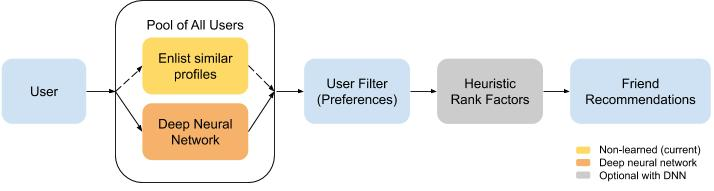
\includegraphics[scale = 0.5]{figures/diagrams/main_flow.jpg}
\caption{Main flow of friendship recommendation system}
\label{fig:mainflow}
\end{figure}

%=====1.3 Report Structure =====
\section{Report Structure}
This thesis is organized as follows. It starts with a background chapter that introduces the basic concepts and the approach towards solving the problem. Further, the findings of our literature study are thoroughly described. Next, chapter 3 introduces the technical and practical methods and its implementation details involved in tackling this problem. In chapter 4, we present the results of the various recommender systems that were developed. It also covers scientific experiments along with analysis of its outcomes. Lastly, chapter 5 and 6 consists of discussion and conclusions encompassing the overall outcome of the project, practical usefulness and its social impacts. In the end, a section is devoted to describing the scope of its future work. Following these will be the references and appendices. 

%=================2.1 Background===================
\chapter{Background}
\section{About GoFrendly}
GoFrendly\footnote{www.gofrendly.se} is an online social networking service exclusively for women. The company was founded in 2016 in Stockholm, Sweden. The word `frend' stands for a person whom you do not know in real life, yet is a friend on the internet\footnote{https://www.urbandictionary.com/define.php?term=Frend}. As of 2020, GoFrendly is a free application and available to the public on Android and iOS devices on selected countries including Sweden, Germany, Norway and India. GoFrendly enables users to find, meet and make friends at ease. GoFrendly enables users to connect with like-minded friends in one's local area and create meaningful friendships. Furthermore, it features personalized matching feed based on one's interests and life situation. It also features discovery of local activities or events such as join or host book reading clubs, cooking workshops, dinner parties or a girls' night out, and meet new women friends who share interests in music, travel, food, arts, yoga, books, photography, movies, hiking and many more. \\

Users can sign-up to create an account on the mobile application at no cost and then, complete their user profile with information such as my\_story, i\_am, meet\_for, marital\_status, kids, age and location. Age and location are numerical data whereas my\_story is a textual data, and lastly, i\_am, meet\_for, marital\_status and kids are categorical data chosen from a list. Further, users set the preferences such as what kind of friends one is looking for and what would one like to meet for. Accordingly, a user can find friends on the platform and meet them in real life. Besides, the application offers many more features to enrich the social experience such as in-app chat service, video call service, social activity finder, activity calendar, and many more interesting features constantly being roll-out for its users.
%visuals
%=====2.2 Recommendation Systems =====
\section{Recommendation Systems}
\subsection{Common Recommendation System Types}
Recommendation models are mainly classified into three categories: collaborative filtering, content-based recommender system, and hybrid recommender system \cite{shuai}. Firstly, Collaborative Filtering (CF) makes recommendation by learning from user's historical interactions; for example, recommending new friends based on current friends circle. However, this mechanism suffers from a cold start problem for new or isolated users wherein the system lacks sufficient information about the user's friends circle to make accurate predictions. Secondly, the content-based recommendation is based primarily on information that users have described about themselves \cite{shuai}. Although this solves the cold start problem, it suffers for incomplete profiles, i.e., the ones with little or no data of the description about themselves. Finally, a hybrid model refers to a recommender system that integrates two or more types of recommendation strategies \cite{shuai}. The hybrid system is proven to be superior in performance and thus, the choice for our case \cite{shuai}.

% Deep learning recommendation systems
\subsection{Deep Learning based Recommender Systems}
In this section, we will understand the reasons for applying deep learning techniques to recommendation systems. Deep learning is generally considered to be a sub-field of machine learning. The typical defining essence of deep learning is that it learns deep representations, i.e., learning multiple levels of representations and abstractions from data. One of the most attractive properties of deep neural architectures is that they are (1) end-to-end differentiable and (2) provide suitable inductive biases catered to the input data type \cite{shuai}. Further, the strengths of deep learning-based recommender systems include (1) nonlinear transformation which enables them to capture complex and intricate user interaction patterns, (2) representation learning which eliminates the expensive feature engineering and enables the models to include heterogeneous content such as numerical, categorical and textual information, and (3) flexibility which comes with the freely available deep learning frameworks such as PyTorch\footnote{www.pytorch.org} which enables efficient and modularized development \cite{shuai}. \\

However, these models do have potential limitations. (1) interpretability: a common argument against deep neural networks is that the hidden weights and activations are generally non-interpretable, limiting explainability. (2) data requirement: deep learning is known to be data-hungry, in the sense that it requires sufficient data in order to fully support its rich parameterization. (3) extensive hyperparameter tuning involved in the deep neural networks. However, these concerns have been fairly addressed with the advent of modern deep neural networks \cite{shuai}. \\

Moreover, deep neural networks offer a vast set of architectures and mechanisms to tackle various recommendation problems. Some of the architectures are as follows: Multi-Layer Perceptron (MLP), transformers, Graph Neural Networks (GNN), auto-encoder, CNN, RNN, Neural Autoregressive Distribution Estimation (NADE), adversarial networks, attentional models, Deep Reinforcement Learning (DRL) \cite{shuai}. Another approach includes context-aware recommendation systems wherein user preferences differ with the context such as time, day, season, mood, place, location \cite{khalid}. Because of all these solid reasons deep neural networks are the first choice of solution for our case. 

%=====2.3 Neural Network =====
\section{Neural Network}
\subsection{Types of Learning Problems}
There are four main types of learning problem in neural networks: supervised, unsupervised, semi-supervised and reinforcement learning. Generally, we categorize a learning problem based on available data and the end goal. \\

Supervised learning describes a class of problem that involves using a model to learn mapping between input examples and its target variable. Here the data consist of input values with definite output labels for each sample. Classification and regression are the common types of problems that are solved by supervised learning methods. On the other hand, unsupervised learning involves using a model for unlabelled data (target variables are not known) to identify patterns and structures present in them. The goal in such unsupervised learning problems may be to discover groups of similar examples within the data, where it is called clustering, or to determine the distribution of data within the input space, known as density estimation, or to project the data from a high-dimensional space down to two or three dimensions. \\

Next, reinforcement learning describes a class of problem that aims at using observations gathered from the interaction with the environment to take actions that would maximize the reward or minimize the risk. Common algorithms include Q-Learning, Temporal Difference (TD), Deep Adversarial Networks. Lastly, Semi-supervised learning describes a problem wherein a small amount of labelled data is available with a large amount of unlabeled data for training as well as testing. Semi-supervised learning falls between unsupervised learning (with unlabelled training data) and supervised learning (with only labelled training data). Our case can be seen as a semi-supervised learning problem as the social relationship between any two parties is either labelled as mutual friends or blocked friends, or unlabelled. 
\subsection{Main Idea}
A social network can be represented in a graph with users as nodes and mutual friendship as edges. Figure 2.1 demonstrates the graph for a sample social network. Henceforth user and node shall be used interchangeably. 

\begin{figure}[h!] %[hbt!]
\centering
\captionsetup{justification=centering}
\includegraphics[scale = 0.5]{figures/diagrams/main_idea.jpg}
\caption{An example of social network graph. (Adapted from \cite{PinSage}.)}
\label{fig:mainflow}
\end{figure}

\newpage

\noindent Our task can be subdivided into two: 
\begin{enumerate}
  \item User Characterization:\\
  To characterize each user based on profile information and friends circle. 
  \item Encoders: \\
  To find pattern between user characteristics and friendship connections.
\end{enumerate}

\subsubsection{User Characterization}
\noindent A rich user characteristics need to include (1) user profile information (node information) (2) user's friends circle (graph structure information or simply graph information). For this case, a model can be classified based on which of these information is used for user characterization. Figure \ref{fig:classification} shows the classification of the models. A random recommender would mean none of the user specific information is used. A non-learned model uses only the user profile information. A Deep Neural Network (DNN) for our case must be capable of incorporating both node information and graph information upto K-degrees. DNN shall be developed as a part of this thesis work. Our focus is mainly on non-learned and DNN models. \\

\begin{figure}[h!]
\centering
\includegraphics[scale = 0.5]{figures/diagrams/classification.jpg}
\caption{Model classification based on information used.}
\label{fig:classification}
\end{figure}

To characterize an user, we need to represent them in a mathematical form for further steps. Firstly, we need to identify relevant methods inclusive of DNNs to mathematically represent user profile information and shall be identified as user/node features henceforth. Secondly, we need to identify relevant methods inclusive of DNNs to mathematically represent user graph structure information. Both of these act as a pointers for our literature study.\\

%==
\subsubsection{Encoders}
\noindent Once rich user characteristics available, we need to encode user characteristics such that a relevance in user characteristics can be associated with friendship compatibility. In particular, we encode each user so that similarity or proximity in a mathematical embedding vector space approximates friendship compatibility in the original network \cite{jure}.\\

Encoder is trained using existing friendship connections. Thereafter, all the users are encoded onto the embedding vector space and what we obtain is called as user embeddings or node embeddings. User embeddings are distinctive numerical vectors that are tagged with each users, which represents its friendship compatibility position in the embedding vector space. Hence, a nearest neighbor search for a chosen user in the embedding space forms a potential friend recommendations. Figure ~\ref{fig:encoder} shows the idea of the described encoder. 

\begin{figure}[h!]
\centering
\includegraphics[scale = 0.55]{figures/diagrams/encoder.jpg}
\caption{Intuition behind an encoder (Adapted from \cite{jure})}
\label{fig:encoder}
\end{figure}

Next section follows a formal literature survey towards finding relevant methods inclusive of deep neural networks to achieve the aforementioned subtasks.

%=====2.4 Previous Work =====
\section{Previous Work}
\subsection{How the study on prestudy work was conducted} 
Google scholar was used as the main search engine. Search keywords such as deep learning, social network, friend recommendation, link prediction and other related specific words in combination are used. Relevant high profile conference publications such as KDD and ECIR were screened and the ones which are peer-reviewed and having significant citations were preferred. Popular research projects such as Stanford Network Analysis Project (SNAP) \cite{snap} were considered. In addition, social network service providers - such as Facebook and Linkedin - recommendation strategies were referred. In addition, several research works have been studied but omitted from this report to maintain brevity and to ensure relevance.

% Academic world
\subsection{Industrial Published Recommendation Methods}
Friendship recommendation is one of the key features of many social network platforms. Social network giants namely Linkedin and Facebook were considered to examine their methods. Recommendation strategies are a secret recipes of the companies, but information on some of the methods in use is publicly made available. However, the performance of their friendship recommendation is not quoted publicly. 

\subsubsection{Linkedin Network Recommendations}
\noindent LinkedIn suggests new network connections under the `People You May Know' feature based on common profile information. Another feature called `People Also Viewed' shows the member profile that the viewers of one's kind have also looked at. The latter strategy may go wrong as the listed profiles may be mistaken to be associated with the visited profile \cite{linkedin}. 

\subsubsection{Facebook Network Recommendations}
\noindent Facebook's `People You May Know' feature recommends new friends and these suggestions are based on factors such having friends in common, from being in the same Facebook group or school or work network and lastly, the contacts that have been uploaded by the user \cite{facebook}. These quoted methods are a non-learned and heuristic methods. Besides, finding new friends is not the top reason users use facebook for. 
\subsection{Academia}
\subsubsection{Referred Conference publications}
\noindent Below follows a list of relevant popular conferences which were referred. 
\begin{enumerate}
    \item SIGIR: Special Interest Group on Information Retrieval.
    \item KDD: Knowledge Discovery in Databases.
    %\item RecSys: Recommendation Systems
    %\item ACM: Association for Computing Machinery
    %\item KDIR: Knowledge Discovery and Information Retrieval
    \item ECIR: European Conference on Information Retrieval.
    %\item CIKM: Conference on Information and Knowledge Management
    \item WWW: International World Wide Web Conference.
    %\item WSDM: Conference on Web Search and Data Mining
    \item ICTIR: International Conference on Theory of Information Retrieval.
\end{enumerate}
\subsubsection{Stanford Network Analysis Project (SNAP)}
\noindent SNAP is an active network analysis research project led by Prof. Jure Leskovec and has highly cited publications. More recent ones involve deep neural network based network analysis methods \cite{PinSage}. Alongside, it hosts several databases related to network analysis for the public, and a general-purpose scalable network analysis library \cite{snap}.
%http://snap.stanford.edu/

% Industrial world
\subsection{Representation of User Profile Information}
The goal is to represent a user's profile in a mathematical vector form and shall be identified as user features here onwards. The user profile information consist of my\_story, i\_am, meet\_for, marital\_status, kids, age and location. Age and geographic location are numerical data and shall be kept as it is whose total vector size is 3. Categorical data are i\_am, meet\_for, marital\_status, kids, which are categorical options chosen from a set of options. Categorical data are one-hot encoded whose total vector size is 45. Figure \ref{fig:user_data} shows the breakup. Furthermore, my\_story is a textual data whose semantics needs to be considered for our case. Now, our focus is on the semantic representation of the user's my\_story. \\

Several advancements have taken place in the last decade in the field of semantic representation of textual data. Various word embeddings mechanisms have been proposed. Introduction of word vectors involving Continuous BoW (CBOW) and SkipGram architectures \cite{skipgram} were the early success in semantic representation of words. Variants of the word vectors are as follows: word2vec from Google \cite{word2vec}, GloVe by Stanford \cite{glove}, and fasttext by Facebook \cite{fasttext}, all of which have shown similar performances. Further step-up in the performance were seen in node2vec architecture, which is based on biased random walk wherein the words are represented in the graph \cite{node2vec}.\\

More recently, language transformers have profoundly improved the estimation of textual semantics. BERT \cite{bert} and RoBERTa \cite{roberta} have set new state-of-the-art performance on semantics of textual data. However, these models involve massive computational overhead in the training setup when run on large-scale datasets. A more recent publication titled Sentence-BERT \cite{sbert}, a modification of the pre-trained BERT network, offers comparable accuracy with significantly fewer computations at inference. In the next section, we introduce the technical details of the SBERT mechanism. % However, these transformers are trained to generate semantic embeddings of single sentence and may underperform when we try to generate semantic embeddings for a group of sentences. However, for simplicity purpose we limit to S-BERT mechanism.\\

\subsubsection{Sentence-BERT Mechanism}
\noindent Sentence-BERT (SBERT) is a modification of the pre-trained BERT network that uses siamese and triplet network structures to derive semantically meaningful sentence embeddings that can be compared using cosine-similarity. This reduces the effort for finding the most similar pair from 65 hours with BERT or RoBERTa to about 5 seconds with SBERT, while maintaining the accuracy from BERT \cite{sbert}. A large disadvantage of the BERT network structure is that no independent sentence embeddings are computed, which makes it difficult to derive sentence embeddings from BERT. To bypass this limitations, SBERT proposes that single sentences are passed through BERT and then employ a pooling layer to derive a fixed sized embedding which then trained in a siamese structure. The parameters of the BERT model are fine-tuned such that the semantically similar sentences are cosine similar in the embedding space. Figure ~\ref{fig:sbert} shows the SBERT architecture. This model is when evaluated on the Semantic Textual Similarity (STS) tasks gives a performance of 86.39\%.

\begin{figure}[h!]
\centering
\includegraphics[scale = 0.28]{figures/diagrams/sbert.PNG}
\caption{SBERT architecture. (Reproduced from \cite{sbert}.)}
\label{fig:sbert}
\end{figure}

\newpage
Pre-trained SBERT model shall be used for our case to extract semantic representations of users' textual data i.e., my\_story. The choice of pre-trained model is ‘roberta-base-nli-stsb-mean-tokens’ which describes that the pre-trained model is RoBERTa base with a mean pooling strategy and fine-tuned for STS (Semantic Textual Similarity) task. The base model provides a fixed vector size of 768. Figure \ref{fig:user_data} enlists all the user profile information along with their values, vector size and corresponding data type. \\

\begin{figure}[h!]
\centering
\includegraphics[scale = 0.5]{figures/diagrams/user_data.jpg}
\caption{Numerical, categorical and semantic data of a user profile}
\label{fig:user_data}
\end{figure}
\subsection{Representation of User Graph Structure Information}
The goal here is to represent the user's friend circle i.e., local neighbourhood of the users in a mathematical form. Just as there have been major advancements in the representation learning on textual data, the representation learning on graphs (Graph Neural Networks) have also have undergone major developments. Moreover, some of these GNNs are capable of incorporating both user features and graph information, and achieve an encoder objective. The encoder objective, as previously described, is to encode the user characteristic such that similarity or proximity in vector embedding space approximates friendship compatibility in original network. In this section we delve into various GNN-based encoders for this case. \\

The notion of neural networks for graph data was first outlined in Gori et al. (2005) \cite{gori} and further elaborated in Scarselli et al. (2009) \cite{scar}. Then, the graph embedding methods such as adjacency-based similarity (2013) \cite{ahd}, multi-hop similarity (2015) \cite{cao}, random walk (2014) \cite{rw} and node2vec (2016) \cite{n2v} showed improvements in learning graph representations. Node2vec has found to perform better on node classification while multi-hop methods for link prediction (2017) \cite{goy}. Node2vec has been fairly successful in generating friend recommendations for a social network graph with heterogeneous edges (2019) \cite{verma}.  However, these encoders have shortcomings such as linear parameter size, cannot incorporate node features, and inherently transductive i.e., it is not straight forward to generate embeddings for new nodes that were not included in the training set.\\

In contrast, deep encoders have shown its prowess to capture the deep representations of graph structures. These encoders rely on the notion of `Graph Convolutions Networks' (GCNs). This approach originated with the work of Bruna et al. (2013) \cite{bruna}, which presented a version of graph convolutions based on spectral graph theory. Following on this work, GCNs have shown new state-of-the-art results on benchmarks such as node classification, link prediction, as well as recommender system tasks (e.g., the MovieLens benchmark \cite{mlens}). Within GCNs, several variants are available such as GraphSAGE (2017) \cite{gsage} and Gated Graph Neural Network (2016) \cite{gate}. \\

A more recent application of Graph Convolution Networks (GCNs) named PinSage \cite{PinSage} has set new benchmark in large-scale recommendation tasks. PinSage research work was a collaborative research between Stanford and Pinterest. It addresses the large-scale item recommendations for the Pinterest platform. PinSage proposes a randow walk based GCN for web-scale recommender systems. Some of the features of PinSage include inductive learning i.e., the ability to generate embeddings for nodes that were not used in the training, the ability to accommodate node features, scalable to large graphs with billions of nodes. PinSage not only produces the graph representation, but also achieves the encode objective of our case. All these merits make PinSage a right choice for our case. Thus, a modified variant of PinSage can be formulated for our case to generate rich embeddings for each user.\\

%=====2.4 Evaluation =====
\subsection{Friendship Recommendations from Embeddings}
The goal here is to use the node embeddings from the GCN to offer friendship recommendations. Intuitively, a nearest neighbor search can be made in the embedding vector space. Thus, for each user we query for K-Nearest-Neighbors on cosine distance metric and get K numbers of friend recommendations. We then evaluate its predicted recommendations against actual friendships formed.
\section{Evaluation}
Evaluation of the model shall be made wherein the time evolution of the data shall be used to define training, validation and test data. This is because to emulate the use case of the recommender system, in which current friendship connections are used to recommend persons who might become a user's friends in the future. More specifically, we will take a number of snapshots of the state of the network, with some time interval between each snapshot. \\

The first snapshot will be used to define training dataset, the second snapshot to define validation dataset, and the third snapshot to define the test dataset. However, the user set is fixed and the new friendships formed in the successive validation set are accounted for evaluation. In other words, friendship recommendation for the user set in the training set is made and evaluated against new friendship formed for this fixed user set in the validation set. \\

Once the development is complete, test set shall be considered to benchmark its final performance. Figure \ref{fig:eval} shows how the evaluation is performed. We begin from a user and query for nearest neighbors on the vector embeddings space giving us top K prediction list. Then, this list is evaluated against actual friends that were formed. \\

\begin{figure}[h!]
\centering
\includegraphics[scale = 0.6]{figures/diagrams/eval.jpg}
\caption{Evaluation of Friendship Predictions}
\label{fig:eval}
\end{figure}\\

\newpage
To quantify the performance of recommendation model, we need to identify relevant evaluation metrics to optimise and to measure the performance of the algorithm. Evaluation of a recommendation can be divided into offline metrics and online metrics. Online metrics provide a measure of the effectiveness of the online recommendation system after the roll-out into production and actual users have interacted with \cite{eval}. Click-through rate and A/B testing are examples of online metrics. Offline metrics provide a measure of the effectiveness of the model during its development. Offline metrics are further categorised based on factors such as relevance and serendipity. Both of these metrics are covered separately in the following subsections. For the sake of simplicity, we will focus only on offline metrics.

\subsection{Metrics of Relevance}
\noindent These metrics measure how accurate the predictions are when compared against actual friendships that were formed in specific duration of time. Some of the metrics of relevance are Mean Average Precision @K (MAP@K), Mean Average Recall @K (MAR@K), hit-rate and Mean Reciprocal Rank (Rank-aware).

\subsubsection{Mean Average Precision @K (or MAP@K)}
\noindent MAP@K gives insight into how relevant the list of recommended friends are i.e., how many top K predicted friendship recommendations were actually formed in the test set \cite{eval}.

\subsubsection{Mean Average Recall @K (or MAR@K)}
\noindent MAR@K gives insight into how well the recommender is able to recall all the friends that a user has actually befriended in the test set i.e., of all the new links formed, how many were predicted correct in the top K recommendations \cite{eval}.
    
\subsubsection{Hit-rate}
\noindent Hit-rate is computed as what fraction of the actual new friends formed were in predicted top K recommendations. Hit-rate can take values between 0 to 100, where 100 implies all of the actual new friends are in top K predicted list. The value decays linearly with missing each actual friend in prediction list. Subsequently, an average value of the hit-rate of all users is considered. K can be set to 500 because this is a good start, this give sufficient number of users for next component in the actual flow shown in figure \ref{fig:mainflow} i.e., filtering by user preferences.

\subsubsection{Mean Reciprocal Rank (MRR)}
\noindent Mean Reciprocal Rank indicates the ranking factor of the relevance ability of a recommendation system and hence, termed as rank-aware metric. For a user, it is the reciprocal index of the first match. The match is when an actual new friend formed is in the top K recommendations made by our model. This is applicable only if there is a match i.e., hit-rate is non-zero. MRR can take values between 0 to 100. Near to 100 imply that the actual new friends were very high up the list of predicted recommendations. The formula is shown as below. $R$\textsubscript{$u$,$f$} is the rank of user $f$ among recommended friends queried for user $u$, $U$ is the pool of all users in which it was queried and $|U|$ is the cardinality of set U \cite{PinSage}. Unlike hit-rate, MRR decays in a multiplicative inverse with each drop in matched rank. %The scaling factor \textit{s} can be used for example s=100 ensures that the difference between rank at 1,000 and rank at 2,000 is still noticeable, instead of being very close to 0.
    \begin{equation}
        MRR = \frac{1}{|U|} \sum_{(u,f)\in U}^{} \frac{1}{R\textsubscript{$u$,$f$}} \\
    \end{equation}

%\end{enumerate}

\newpage
\subsection{Metrics of Serendipity}
Metrics of serendipity indicates how interesting a recommendation list is. Even if the metrics of relevance is good, we may face the problems such as recommending same set of friends to all users or that the recommendation list is homogeneous (not diversified) or that it shows the same list for a given user every single time \cite{serene}. There are research works that illustrate how focusing on accuracy can actually be detrimental to a recommender system \cite{sean}. Examples are diversity, novelty, and unexpectedness. Diversity metric enforces the variety in any recommendation list. Novelty metric enforces that a list is personalized i.e., different for different users. Unexpectedness enforces that a new recommendation is different from a previous recommendation.\\

However, for the sake of simplicity we focus on offline metrics mainly the metrics-of-relevance (accuracy metrics) for our case. The reason is accuracy metrics are foremost essential to understand the accuracy prediction. And our choices are hit-rate and mean reciprocal rank. Because these are the accuracy metrics that were considered in the research paper PinSage \cite{PinSage} on which our recommendation system is based. Further, hit-rate gives the picture about how accurate the predictions are while MRR gives ranking ability of the prediction accuracy. Both of these together give a fair idea about the ability of our recommendation model. \\

\subsection{Embedding Similarity Distribution}
Another indication of the effectiveness of the learned embeddings is that the distance between random pairs of user embeddings are widely distributed \cite{PinSage}. If all users are at about the same distance (i.e., the distances are tightly clustered) then the embedding space does not have enough “resolution” to distinguish between users of different relevance. Embedding similarity distribution gives a plot of cosine similarity between random pairs of user embeddings.\\

Another indicator of the effectiveness of learned embeddings is `kurtosis'. Kurtosis is a measures the "fatness"  of the tails of a distribution. Excess kurtosis indicate how fat the distribution is when compared against unit normal distribution. Figure  \ref{fig:kurt} shows the values of excess kurtosis for various curves. Excess kurtosis value is 0 for a unit normal distribution which can be seen in black color. The steeper the curve is, the higher the excess kurtosis value is.

\begin{figure}[h!]
\centering
\captionsetup{justification=centering}
\includegraphics[scale = 0.6]{figures/diagrams/kurtosis.png}
\caption{Distribution plot with excess kurtosis value. \\
(Reproduced from \cite{wkurt}.)}
\label{fig:kurt}
\end{figure}
%==================================================================




%=====2.4 Recommendations =====

%================ 3. Methods =================
\chapter{Methods}
In this chapter, we present several methods that are used to solve this problem.
\section{Data Pipeline}
In computing, a pipeline, also known as a data pipeline, is a set of data processing elements connected in series. Figure \ref{fig:pipe} shows the proposed data pipeline for recommendation system. It involves several stages: data collection, data preparation, model training, generation of user embeddings, friend recommendations and lastly, the feedback to model training stage from the model evaluation. Infact, this pipeline can seamlessly undergo all these stages and generate new embeddings on-demand, especially, as and when a new user enters the system. Further, the performance can be periodically monitored which also serves as a decision for the model training. That means suppose the performance is not satisfactory, we may fine-tune the model on-demand. Each stage of the data pipeline is explained in the following section.

\begin{figure}[h!]
\centering
\includegraphics[scale = 0.42]{figures/diagrams/pipe.jpg}
\caption{Data pipeline of friend recommendation system}
\label{fig:pipe}
\end{figure}

\subsection{Data Collection}
As discussed in the evaluation section, we consider three time-series snapshot of the state of the social network from the SQL database, with the specific time interval between each snapshot. The first snapshot is taken on $07^{th}$ of April 2020 and shall be used to define training dataset. The second snapshot is taken a month after on $07^{th}$ of May 2020 and shall be used to define validation dataset. Lastly, the third snapshot is taken three months after on $07^{th}$ August 2020 and shall be used to define test dataset.

\subsection{Data Preparation}
\subsubsection{Data Retrieval}
\noindent Data retrieval means obtaining relevant data from a database management system. Once we get the SQL dump, we setup a local SQL server and perform relevant query using SQL scripts. The query is to extract user profile information such as my\_story, i\_am, meet\_for, marital\_status, kids, birthday and location. The query also involves gathering a list of mutual friends and blocked user pairs on the platform. For the retrieval, we use the softwares such as `SQL workbench' tool to setup local SQL server, `DBeaver' as a SQL client software to interact with the data, and `pymysql' library to import data into our development environment as `Pandas' dataframe and save the files in the HDF5 (Hierarchical Data Format) for further access. 
\subsubsection{Data Organize}
\noindent Data organizing is the process of preparing data for analysis by rearranging, segregation, aggregation, ordering, or modifying the structure of data that is cluttered or disintegrated. Raw data may hold data in multiple columns or may have in randomly ordered, etc.. Once the raw data has been obtained, we may need to organize the data. This includes subtasks such as segregation, aggregation, ordering and formatting. In the end, we obtain two sets of data. One is the organised user profile information, and two is the list of mutual friends and blocked user pairs.

\subsubsection{Data Cleansing}
\noindent Data cleaning is the process of preparing data for analysis by filtering or modifying data that is incorrect, incomplete, irrelevant, duplicated, or improperly formatted. These type of data are not helpful when it comes to analyzing them and it may hinder the process or provide inaccurate results. We carry-out operations such as imputation i.e., assign default values to missing or erroneous values, removal of duplicates, emoticons and multiple punctuation marks from the textual data.

\subsubsection{Data Transformation}
\noindent Data transformation is the process of converting a raw data source into a transformed, validated, and ready-to-use form. We transform numerical, categorical and semantics data into mathematical features. The categorical data into one-hot encoded vector while the numerical data is kept as it is. More importantly, the user profile is in different languages because of the global userbase who prefer to have the profile in their local languages. Although numerical and categorical data can be mapped directly from local language to user features, the textual data needs to be translated to a unified lingo which is chosen to be English. Hence, we translate all the users story to English language so that we can use available pre-trained SBERT model to generate semantic embeddings. We used Google Cloud Platform (GCP) Translator API service for the translation. However, due to the high cost price of the GCP translator service, we consider only the Stockholm city users for our experiments that includes user semantics which accounts to 14,948 users. 

%\chapter{Models}
\section{Non-learned Recommender System}
The current friend recommendation system at goFrendly is a non-learned system which was developed based on intuition. It enlists similar users based on profile information. This is achieved by computing k nearest neighbors on cosine metric for users. In other words, the user features form the user embeddings directly. \\

%\section{Neural Network 01 (A Simple Encoder)}
%\subsection{Neural Network Algorithm}
%\subsection{Hyperparameters}
%\subsection{Loss Function}
\section{GCN-based Encoder}
\subsection{Graph Convolution Network}
Graph convolution networks involve generation of user embeddings for a chosen target node from its node features and graph structure information. GCNs are known to produce rich embeddings compared to other graph embedding methods. Each successive degree connections of the node become a sequentially connected layer in its computational graph. It begins from the user features and undergoes neural operations getting transformed and aggregated across several layers (deep layers). The information flows from K-degree connections towards the target node thereby capturing the deep representations of the node's neighborhood. \\

Figure \ref{fig:gnn} demonstrate the idea of GCN. On the left side, a sample input graph is considered wherein neighborhood aggregation is performed for the target user node A. On the right side, we have the computation graph wherein each successive layer from node A represents its k-th degree connections. Here, Layer-2 represent the target user node, Layer-1 is its first degree connections, and Layer-0 is its second degree connections. The layers are named in the reverse order for the mathematical convenience. The user features in the Layer-0 gets transformed, aggregated and propagates across layers and forms the embedding of the target user node. In general, Layer-K represents the target node while Layer-(K-1) represent its first degree connections, and Layer-0 its Kth-degree connections. However, the computational graph and aggregation function can be defined in several ways which shall be discussed in the next subsection. \\

\begin{figure}[h!]
\centering
\captionsetup{justification=centering}
\includegraphics[scale = 0.6]{figures/diagrams/gnn.jpg}
\caption{(1) A sample input graph with a target node A (left diagram), \\ (2) Demonstration of GCN on node A (right diagram) (Adapted from \cite{PinSage}). }
\label{fig:gnn}
\end{figure}
\subsection{PinSage}
PinSage mechanism provides the techniques involving computational graph formation and aggregate function for our GCN algorithm \cite{PinSage}. \\

\noindent Key techniques proposed in PinSage that shall be used for our problem:
\begin{enumerate}
    \item Random walk based computation graph for each node.
    \item On-the-fly convolutions
    \item Importance pooling of neighborhood.
\end{enumerate}

Figure \ref{fig:algo} shows the overview of our neural network system. We begin from the user input features and mutual friends list, then create a social network graph. Thereafter, random walk is carried-out for each node upon which K-layers computation graph is formulated. Starting from user features the PinSage convolution is applied onto each node's computation graphs yielding us with node embeddings. The operations such as random walk and PinConv shall be specifically explained in the next section.

\begin{figure}[h!]
\centering
\includegraphics[scale = 0.5]{figures/diagrams/gcn.jpg}
\caption{Neural Network Model involving PinSage based GCN.}
\label{fig:algo}
\end{figure}

\subsubsection{Random Walk}
\noindent Computational graph for our convolution algorithm is based on random walk. Random walk gives the importance-based local neighborhood, where the neighborhood of node $u$ is defined as the $T$ nodes that exert the most influence on node $u$. Random walk is simulated starting from node $u$ and compute the visit count of nodes tread by the random walk. Random walk parameters include number of walks, length of walks, and number of neighbors. These parameters are the hyperparameters of a random walk. An example of random walk is shown in figure \ref{fig:rw}.\\

\newpage

\begin{figure}[h!]
\centering
\captionsetup{justification=centering}
\includegraphics[scale = 0.4]{figures/diagrams/rw.jpg}
\caption{An example of Random Walk operation. (Adapted from \cite{PinSage}.)}
\label{fig:rw}
\end{figure}

We have considered a small input graph and random walk shall be performed for the target node A. Its parameter values be chosen as (1) length of walk = 6, (2) number of walk = 1, (3) number of neighbors = 3. Then, top 3 most visited nodes are considered with its visit counts as the weights. The obtained computational graph along with its weights for our target node A is shown on the far right diagram. With longer walks, far neighborhood can be spanned while more number of walks lead to larger coverage of nearby nodes. However, a large number of neighbors would sometime mean more similar neighbor nodes for many nodes. Thus, the choice of random walk parameters is important which shall be selected from hyperparameter tuning.

\subsubsection{PinConv}
\noindent PinConv, a variant of GCN, performs an efficient localized convolution by sampling the local neighborhood of a node. Algorithm 1 below describes the mathematical details of the aggregate function proposed in PinSage \cite{PinSage}. We consider the task of generating an embedding, $z_u$ for a node $u$, which depends on the user’s features and the graph structure around this user node $u$. This procedure is detailed in Algorithm 1. The basic idea is that we neural transform the representations $z_v$, $\forall v \in N(u)$ where $N(u)$ represents $u$’s neighbors, through a dense neural network and then apply an aggregator/pooling function (e.g., a element-wise mean or weighted sum, denoted as $\gamma$) on the resulting vectors (Line 1). This aggregation step provides a vector representation, $n_u$, of $u$’s local neighborhood, N($u$). We then concatenate the aggregated neighborhood vector $n_u$ with user $u$’s features $h_u$ and neural transform through another dense neural network layer (Line 2). Additionally, the normalization in Line 3 makes the training more stable, and it is more efficient to perform an approximate nearest neighbor search for normalized embeddings. \\

\begin{figure}[h!]
\centering
\captionsetup{justification=centering}
\includegraphics[scale = 0.4]{figures/diagrams/pinconv.PNG}
%\caption{(Adapted from \cite{PinSage})}
\label{fig:pinconv}
\end{figure}
\section{Model Training}
Figure \ref{fig:train} shows the model training. User features and mutual friends undergo neural network operation as described previously in figure \ref{fig:algo}. Then, the model produces user embeddings for which loss value is computed using  mutual friend and blocked user pairs. Later, we carry-out back propagation algorithm to update the model parameters.

\begin{figure}[h!]
\centering
\includegraphics[scale = 0.5]{figures/diagrams/train.jpg}
\caption{Model Training}
\label{fig:train}
\end{figure}

\subsection{Loss Function}
The loss function for the training of our neural network model is cosine embedding loss. Cosine embedding loss optimises the neural network to generate embeddings such that the embeddings of the mutual friends are brought closer while the blocked users are pushed apart. The equation of cosine embedding loss function is shown in figure \ref{fig:closs}. Suppose $x_1$ and $x_2$ are the user pair while $y$'s value represents whether they are friends or blocked users. Margin or also called as loss margin indicate the magnitude of push for the negative user pairs. \\

\begin{figure}[h!]
\centering
\[
    Loss(x,y)= 
\begin{dcases}
    1-cos(x_1, x_2), & \text{if } y = 1\\
    max(0, cos(x_1, x_2) - margin), & \text{if } y = -1
\end{dcases}
\]
\caption{Cosine Embedding Loss function}
\label{fig:closs}
\end{figure}

\subsection{Hyperparameters}
In this entire setup we have several hyperparameters, which we shall divide further based on operations as follows.

\subsubsection{Hyper parameters 01 (Random walk parameters)}
\noindent These hyperparameters are related to random walk operation. The hyperparameters are the number of walks, length of walk and number of neighbors for each node.

\subsubsection{Hyper parameters 02 (Model configurations)}
\noindent These parameters are related to neural network configurations. The model configuration parameters are the dimensions of convolutional layers, number of hidden layers, size of output node embeddings.

\subsubsection{Hyper parameters 03 (Model training)}
\noindent These parameters are related to neural network training operation. The model training hyperparameters include parameters such as loss margin, learning optimizer and learning rate. 

\subsection{Hyperparameter Tuning}
In order to identify optimal model configurations, we carried-out hyperparameter tuning. Figure \ref{fig:hype} shows the range of values that were tried to find the optimal values. The range is denoted with square brackets wherein the choice was a randomly picked value in the given range. Tuning was carried-out one variable at a time. The figure also shows the chosen values that performed the best.

\begin{figure}[h!]
\centering
\includegraphics[scale = 0.5]{figures/diagrams/hype.jpg}
\caption{Hyperparameters with its experiment values and its chosen value.}
\label{fig:hype}
\end{figure}

%=================={Results and Analysis==============================
\chapter{Results and Analysis}
In this section, we shall benchmark the performance of three recommendation models. The models are random recommender system, non-learned recommender system and GCN recommender system.
\section{A Random Recommender System}
At first, we evaluate the random recommender system which neither uses user profile information nor its friend circle information. Hence, the user embeddings are uniformly randomly initialized. A uniform random recommender would mean selecting 500 users from 14,948 (Stockholm city) users at random that approximately translates to 3.33 in hit-rate and 0.66 in MRR. 
\section{Non-learned Recommender System}
As mentioned earlier, a non-learned recommender system enlists similar profile which is implemented by k nearest neighbors on the user input features. Figure \ref{fig:nl} shows the non-learned recommender performance for numerical, categorical and semantic data individually and all in combination. 

\begin{figure}[h!]
\centering
\includegraphics[scale = 0.45]{figures/diagrams/nonlearned.jpg}
\caption{Non-learned recommender system performance.}
\label{fig:nl}
\end{figure}

From the above results, we may notice that each data class has shown different performances. Non-learned model is well generalized as the performance on training and validation data is comparable for all data classes. However, numerical data tops in performance by a significant value compared to others. This shows that numerical data have a direct influence on the friendship formed. In other words, the users who are friends are closer on `age' and `location' values than other features. \\

Further, to get an idea about the distribution of these features we shall plot the embedding similarity distribution individually for each class and in combination of all class. Figure \ref{fig:nled} shows the plot. Further, excess kurtosis values for each have been computed and are 10.77, 1.03, -1.24, 4.44 respectively. Numerical data are clustered close to 1 with kurtosis indicating highest steepness whereas semantics data less clustered with least kurtosis value. In general, wider curves with lesser kurtosis are preferred as they are known to have better resolution. However, our results indicate otherwise i.e., higher kurtosis data has higher performance while lower kurtosis data has lower performance. \\


\begin{figure}[h!]
\centering
\includegraphics[scale = 0.6]{figures/diagrams/nl_ed.jpg}
\caption{Embedding similarity distribution of the user features}
\label{fig:nled}
\end{figure}

More specifically, the current recommendation system at GoFrendly combines numerical(3) and categorical(45) data alone. Numerical data consists of `age' and `location' whereas categorical data consists of ‘i\_am’, ‘meet\_for’, ‘marital\_status’, ‘kids’. Thus, we shall benchmark the results for these two cases and later extend to include semantics data. As we have the semantics data of Stockholm city users alone, our user size here is 14,948. Figure \ref{fig:nl2} shows the performance of random recommender as well as the non-learned system for the same. \\

%numerical data consists of `age' and `location', categorical data consists of ‘i\_am’, ‘meet\_for’, ‘marital\_status’, ‘kids’, and semantic data consist of `my\_story'. numerical and categorical data alone viz. ‘i\_am’, ‘meet\_for’, ‘marital\_status’, ‘kids’, ‘age’ and ‘location’. It does not include textual data or stories.

\begin{figure}[h!]
\centering
\includegraphics[scale = 0.5]{figures/diagrams/nl2.jpg}
\caption{Performance of random and non-learned models}
\label{fig:nl2}
\end{figure}

It is evident from the figure that the non-learned recommender system performs significantly better. It is worthwhile to note that the model has excellent generalization i.e., the performance on the validation data was compared with the performance on the training data. The loss value was found to be 0.089. In the next section, we shall develop a deep graph neural network-based encoder to generate rich user embeddings and compare with its performance.

%\section{Neural Network 01 (A Simple Encoder)}
%\section{Neural Network 02 (A GCN-based Encoder)}
\section{GCN-based encoder} \label{gcn}
Our PinSage based GCN model underwent training with user features as initial node embeddings. The user features size was 48 while the users set was limited to Stockholm city i.e., 14,948. Figure \ref{fig:pipe} shows the data pipeline and describes how the training is carried out. The hyperparameter values are chosen from its tuning shows in figure \ref{fig:hype}. The parameter values are length of random walk = 64, number of random walks = 32, number of neighbors = 16, learning rate = 3e-4, optimizer = ‘RMSprop’, loss margin = 0.25, dimension of convolution layer = 48, number of hidden layers = 0, user embeddings size = 48, and training samples = mutual friends and blocked pairs. \\

Figure \ref{fig:gcn1a} shows the loss values over the course of training. The green line overlay represents the loss value of the non-learned system. It is noticeable that the value reduced smoothing affirming the choice of our training optimizer and learning rate. The training consisted of 9,745 trainable model parameters for this case. \\

\begin{figure}[h!]
\centering
\includegraphics[scale = 0.55]{figures/diagrams/gcn1a.jpg}
\caption{Loss values during model training}
\label{fig:gcn1a}
\end{figure}

\newpage

Figure \ref{fig:gcn1b} shows the model's hit-rate and MRR with respect to training epochs. It is worth noticing that the hit-rate and MRR have gradually improved over the course of training and reached a new benchmark. However, the performance gap between training and validation indicate overfitting. Generalization techniques such as including layers of dropout, reducing the number of hidden layers, and early stopping were already been worked out. All these attempts had reduced the training-validation curve gap and the best was presented here in figure \ref{fig:gcn1b}. However, further generalization could not be achieved. \\

\begin{figure}[h!]
\centering
\includegraphics[scale = 0.55]{figures/diagrams/gcn1b.jpg}
\caption{Hit-rate and Mean Reciprocal Rank (MRR) during training. }
\label{fig:gcn1b}
\end{figure}

The green line overlay represents the performance of the non-learned system on the validation dataset and a baseline for our comparison. The best Hit-rate (marked with a blacked circle) were seen to be 52.0 and 34.1 on training and validation data respectively. Both of these values surpass the non-learned recommender system by a huge margin. Furthermore, the top value of MRR was 4.8 and 1.0 on training and validation data respectively. Although MRR has risen for the training data, it has shown no improvement for the validation dataset compared against non-learned MRR. Thus, the model state where its node embedding produced highest hit-rate on validation data is considered. \\

Moreover, to understand the evolution of the distribution of user embeddings with training epochs, we shall plot its embedding similarity distribution taken at regular epoch intervals. Figure \ref{fig:embdist} depicts the embedding similarity distribution. We observe top performance at epoch 400. Although the curves have a similar distribution, we may notice that embeddings corresponding to epoch 400 are more clustered (less wide) than others. Besides, excess kurtosis were computed and were -1.44, -1.45, -1.51, -1.49 for epoch 100, 200, 300 and 400 respectively. Excess kurtosis values are almost the same to compare and deduce. All these observations coupled with our previous observation in figure \ref{fig:nled} indicate that embedding similarity distribution and kurtosis values are not positively correlated with the model's performance. \\

% Number of model parameters: 9745, 2672401
\begin{figure}[h!]
\centering
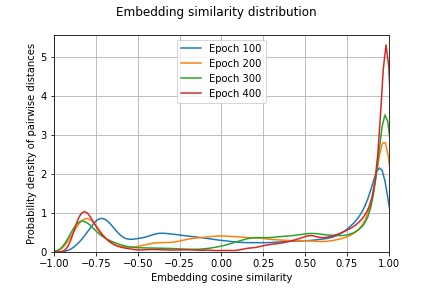
\includegraphics[scale = 0.55]{figures/diagrams/one_embdist.jpg}
\caption{Similarity distribution of the GCN produced user embeddings}
\label{fig:embdist}
\end{figure}
\section{Models Comparison}
Figure \ref{fig:mcomp} compares the performance between non-learned and GCN-based recommender system. It is evident that GCN architecture allowed the model to capture the friendship patterns well leading to almost twice as non-learned model's performance on both hit-rate and MRR for training data. Furthermore, the hit-rate improvement on validation dataset is significant by 29.16\% over non-learned. However, no significant improvement in MRR for the validation data was noticed.

\begin{figure}[h!]
\centering
\includegraphics[scale = 0.55]{figures/diagrams/mcomp.jpg}
\caption{Comparison between non-learned model and GCN model}
\label{fig:mcomp}
\end{figure}
\section{Experiments}
In order to improve the performance, for the same GCN design we shall carry-out experiments such as (1) include user semantics information and (2) increase the training userset to users of all cities.
\subsection{Include User Semantics information}
In this case, we extend the user features to include numerical, categorical, and semantics data with a data size of 3, 45, and 768 respectively. User features now consist of my\_story, i\_am, meet\_for, marital status, kids, age and location leading to a total of 816 vector size. However, the user size is fixed to Stockholm city users. \\

\begin{figure}[h!]
\centering
\includegraphics[scale = 0.55]{figures/diagrams/gcn2a.jpg}
\caption{Loss values}
\label{fig:gcn2a}
\end{figure}

The training consisted of 2,672,401 trainable model parameters for this case. The choice of hyperparameters was the same except the learning rate which was 1e-5. Figure \ref{fig:gcn2a} shows the loss values during the training. The green line overlay indicates the loss value of our best performing GCN model so far (presented in section \ref{gcn}). Once again, the training was smooth and credits our choice of learning rate and optimizer. Figure \ref{fig:gcn2b} shows the hit-rate and MRR during the training. Looking at both the plots, we can notice that the hit-rate and MRR have scaled new benchmarks. This proves that with rich user features, the model was better able to identify its pattern with friendship formation. However, the model has not performed very well on the generalization as we see a big gap between these curves. Although generalization techniques have already been applied, no further improvements could be made. \\

\begin{figure}[h!]
\centering
\includegraphics[scale = 0.5]{figures/diagrams/gcn2b.jpg}
\caption{Hit-rate and Mean Reciprocal Rank (MRR) during training.}
\label{fig:gcn2b}
\end{figure}

Furthermore, the hit-rate seems to oscillate around 34 whereas MRR has stayed near to 1 over the course of training. A well trained-model is one which performs the best on the validation dataset. Hence, our choice of node embeddings is training epoch 60 (marked with a blacked circle) with hitrate = 65.6, MRR = 8.6 on the training dataset, and Hitrate = 34.6, MRR = 1.4 on the validation dataset. Both of these results outperform our previous GCN setup. 
\subsection{Include All Users of the Platform in the Training} %121109
In this case, we extend the training userset to include users of all cities. The user features now include numerical and categorical data with a vector size of 3 and 45 respectively. User features now consist of \st{my\_story}, i\_am, meet\_for, marital status, kids, age and location. Our evaluation remains to be on the Stockholm city users. \\

\begin{figure}[h!]
\centering
\includegraphics[scale = 0.55]{figures/diagrams/gcn3a.jpg}
\caption{Loss values during training}
\label{fig:gcn3a}
\end{figure}

The training consisted of 9,745 trainable model parameters for this case. The choice of hyperparameters was the same except the learning rate which was 4e-4. Figure \ref{fig:gcn3a} shows the loss values during the training. The green line overlay indicates the loss value of our first GCN model (presented in section \ref{gcn}) at its optimal performance. Once again, the training was smooth and credits our choice of learning rate and optimizer. Figure \ref{fig:gcn3b} shows the hit-rate and MRR during the training. Looking at both the plots, we can notice that the hit-rate and MRR have not performed better than our previous GCN benchmark. Although the hit-rate has improved over the course of training, its best value (marked with a blacked circle) on validation dataset is much lower than the previous GCN's benchmark. Further, MRR, yet again, has remained almost the same. However, we observe that this model is better generalized than the previous one as the gap between training and validation performance is seen to be smaller. \\

\begin{figure}[h!]
\centering
\includegraphics[scale = 0.5]{figures/diagrams/gcn3b.jpg}
\caption{Hit-rate and Mean Reciprocal Rank (MRR) during training.}
\label{fig:gcn3b}
\end{figure}

A well trained-model is one which performs the best on the validation dataset. Since the MRR has remained almost the same. The best result is hitrate = 34.8, MRR = 2.6 on training dataset, and hitrate = 29.2, MRR = 0.9 on validation dataset. Both of these results underperform when compared with our previous GCN setup. On the whole, training the model individually in a particular city is a better strategy than to train on all the cities.

\section{Models Comparison}
So far, we have had two different models viz. non-learned recommendation system and GCN-based recommendation system. And we had three different setups (1) limited user features trained on Stockholm city users, (2) rich user features trained on Stockholm city users, and (3) limited user features trained on users of all cities. Figure \ref{fig:emc1} shows the performance of both these models on three different setups.  \\

\begin{figure}[h!]
\centering
\captionsetup{justification=centering}
\includegraphics[scale = 0.45]{figures/diagrams/emc1.jpg}
\caption{Comparison between non-learned model\\ and GCN model for three different cases.}
\label{fig:emc1}
\end{figure}

From these results, we may deduce that a non-learned model performs best on limited user features for a chosen city, which is the current recommendation system at GoFrendly. However, GCN-based recommendation system significantly outperforms the non-learned system for the same case. For this GCN model, the setup with rich user features trained on a single city yields the top performance. Thus, we may conclude that a GCN-based model performs better than the non-learned model. Intuitively if the evaluation is made by offering to all users of all cities, the model will have a large pool of users to choose from which reduces its performance. This was also seen to be the case when evaluated. Furthermore, we can also deduce that individual encoder for each city can be developed for optimal performance. Lastly, we observe an excellent performance by GCN on training data which suggests that there is a huge scope to improve the model's generalization.\\
\section{Timing Profile}
In all the aforementioned setups training and evaluation took a notable amount of time and figure \ref{fig:time} shows the timing profile. \\

\begin{figure}[h!]
\centering
\includegraphics[scale = 0.45]{figures/diagrams/time.jpg}
\caption{Timing profile of GCN model.}
\label{fig:time}
\end{figure}

From the above figure, we can notice that the time taken by the CPU is multi-fold when compared to GPU. Training time would translate to large time when trained for 100s of epochs. In the case of CPU, we observe that the increase in feature size by a factor of 17 increased the training time by close to 17 times. Similarly is the case for the large training user size. Time taken for the recommendations reflected a factor of 10 multi-fold. \\

However, to speed-up, the tensors were pushed to GPU to compute \& relevant algorithmic functions were changed to PyTorch code. Thus, yielding significant optimization in time. In the case of GPU, we observe that the increase in feature size led to a slight jump in training time whereas the training time for the large users' case was significant. The shown GPU timing is for Nvidia K80; however, when we considered Nvidia P100 GPU, the time reduced further by half. This demonstrates the merits of using GPUs for neural networks. Due to the availability of free GPU resources\footnote{https://colab.research.google.com/notebooks/intro.ipynb} and its computational merits, GPU for training neural networks would just become a norm soon. \\


\newpage
\section{Evaluation on the Test Data}
Now, we consider the test data and evaluate our model performance. Figure \ref{fig:emc2} enlists the values for non-learned and GCN models for three different cases. The underlined values are the top-performing cases. The results on test data is similar to the the results on validation data i.e., GCN model for Stockholm city outperforms non-learned system on both hit-rate and MRR. Performance gain between non-learned and GCN model is shown. \\

\begin{figure}[h!]
\centering
\captionsetup{justification=centering}
\includegraphics[scale = 0.45]{figures/diagrams/emc2.jpg}
\caption{Performance gain between non-learned \\ and GCN model on test data.}
\label{fig:emc2}
\end{figure}

GCN model with full feature size trained on Stockholm city users tops the performance and gives major leap in performance on hit-rate and MRR at 70.8\% and 67\% respectively. GCN model with limited feature size for the Stockholm city yields a moderate gain of 18.9\% and 9\% on Hit-rate and MRR. Lastly, the GCN model with limited features trained on all cities does not perform well enough and it proves that GCN model for each individual city is a better design. Finally, the comparison of the current goFrendly recommendation system which uses limited features size against our top performing GCN model shows that we achieve a gain of 26.9\% on hit-rate and 36.4\% on MRR (highlighted in black boxes). On the whole, our results demonstrate the merit of GCN model in recommending individual friendships. \\

%\section{Practical Aspects}
%\blindtext
%=======================Discussion======================

\chapter{Discussion and Conclusions}
This chapter presents a discussion and conclusions on the outcomes of our research work. It begins with a general discussion about the overall conduct of the thesis work. Then, the practical usefulness of the work along with societal, ethical and sustainability aspects in the real world are described. Thereafter, the conclusions based on the outcomes of this thesis work is presented. Lastly, we shall discuss the scope for further studies and research that are can pursue based on this research work.

\section{General Discussion}
The thesis started with a clear research question 'Can a suitable scalable deep neural network perform better than a non-learned friendship recommender for a given social network, and, if so, by how much?'. To test this hypothesis, we benchmark the performances of non-learned system and deep neural networks and then compare them on a common evaluation metric. At the start, the social network platform did not have pre-existing recommendation data pipeline. \\

In the literature study, we reviewed several methods on the lines of deep neural networks and recommendation systems. More emphasis was given for state-of-the-art methods to solve this case. Our study led to the choice of relevant and essential evaluation metrics. The non-learned recommender system was developed and its performance was recorded. Our study also led to the shortlisting of using pre-trained SBERT language model and PinSage graph network model considering their recent successes. PinSage is a paper from top conference KDD with over 450 citations and it is a modern high-performance graph convolution network applied for a large-scale recommendation. PinSage model was modified to have our loss function. \\

We developed the recommendation pipeline with well-defined evaluation metrics. The proposed data pipeline is flexible to operate on-demand. Then, we trained our PinSage model iteratively by monitoring its prediction performance. The flexibility of our model allowed us to experiment with different setups leading to two more major experiments whose findings showed that a GCN model with full feature size trained for a single city gives optimal performance. Our results demonstrate the merit of GCN in offering friendship recommendations and speaks for itself when it comes to its future potential.

\subsection{Push and Pull Problem}
Another interesting observation during the model training was the phenomenon of push and pull problem. Our loss function was designed to pull the embeddings of mutual friends (positive sample) closer and push the embeddings of blocked user pairs (negative samples). However, if a user pulls two of his friends closer who are blocked users with each other, then the placement of these users in the embedding cannot be successfully placed. This phenomenon could reduce the performance of the model for such cases. This, however, can be solved by having an individual model for each user wherein its positive and negative samples are mutually exclusive. Although the individually trained model is computationally expensive, we only need to train once for each user and thereafter fine-tune on this model would suffice.

\subsection{MLP as a Solution}
Since our PinSage based GCN model was technically complex to build and train, we developed a multi-layer perceptron based encoder as a start to study the compatibility of our recommendation data pipeline with neural network models and also, to ensure smooth training for our chosen loss function. This model is capable of incorporating user features and 1\textsuperscript{st} degree connections and achieve the encoder objective. The model was a multi-layered perceptron with ReLU activation layers and batch normalization. The model was trained for the case of Stockholm city users with limited user features. After the hyperparameter tuning, we obtained a top performance of hit-rate of 27.4, MRR of 1.7 on training data, and hit-rate of 27.1, MRR of 0.8 on validation data. This performance is comparable with the non-learned system. We dismissed any further experiments on this model and considered PinSage based GCN for our further experiments.

\section{Practical Usefulness}
Our results have shown good performance on the offline prediction accuracy metrics. Although accuracy metrics are foremost essential metrics for recommendation systems, it does not suffice to be called as an excellent recommendation system. Study shows that being accurate is not enough and using accuracy metrics alone may hurt the recommender systems \cite{sean}. Other metrics such as metrics of serendipity and online metrics are important to be in place. Our data pipeline and GCN model provides a reliable framework for further developments in the recommendation system. \\

The ranking ability of our GCN based recommendation model has remained a single-digit performance. If this is not satisfactory, we could use the GCN predictions as a user pool and rearrange them based on the heuristic ranking model, which is currently in use at goFrendly. Another point is that our recommender system is trained to capture the friendship patterns seen in a particular city. However, if an individuals friendship pattern differs from the city's crowd pattern, it could be a downside for such minority. In such cases, an individual friendship recommender trained exclusively on each user might solve this shortfall.

\section{Societal, Sustainable and Ethical Implications}
Going by the results, it interesting to witness the model deployed in the real world. With a better performance than its predecessor and the ability to iteratively learn, it is evident that such models shall be eventually deployed in the near future. Also, this is a stepping stone for the developments of several other related features such as the recommendation of entities such as social activities. \\

Friendship recommendation systems are proven to boost user satisfaction leading to user retention and also known to provide user personalization which leads to users in a better mood to use the services  \cite{bval}. Therefore, this research work directly addresses the business value of social network service providers and in turn, it addresses the economic aspects of our society. One of the core services of any social network platform is to facilitate the social dynamics of its user community and our friendship recommender system is one such facilitator. This features specifically benefits users who specifically log into the platform to find friends shall find it with much ease than the previous method. Hence, the societal implications are positive.\\

For the recommendations to thrive and receive appreciations from its users, it has to ensure the lists are interesting. This leads us to focus on metrics of serendipity and regular fine-tuning of the models. With a fair value of diversity, novelty and unexpectedness coupled with regular fine-tuning, the model shall be able to sustain the interest of its users for the longest. In contrast, rendering such elegant and accurate predictions would translate to a lot of cost and computing resources. The computing resources contribute to global CO2 emissions. However, the growing interest among the cloud computing service providers to reduce carbon footprint by methods such as usage of renewable energy takes us a step closer to sustainable future.\\

Users need to allow their personal information to be used to offer them valuable services such as friendship recommendations in return. Without such useful information, the model gives poor results as seen in random recommender system. The current non-learned system at goFrendly uses profile information to offer recommendations. Our model, in addition, uses only the friends circle information of each user and hence, only this information is to be notified to the user for approval. It is important that the privacy of all the users are to be protected. On the ethical aspect, the entire research work was carried out with utmost regards to user privacy and hence, its deployment would also ensure that user privacy is protected. In this regard, users need to be informed that their personal information shall be used regularly to better the service (to fine-tune our models) offered to them and is protected.

\section{Conclusions}
This thesis was an effort towards research and development of friendship recommendation engine for the social network `goFrendly'. In particular, to identify and apply state-of-the-art methods available in the field of recommendation systems. The data considered was a snapshot of the social network. The data had to be organized, cleaned and transformed. Our prestudy involved review of the recent technological advancements in this field and our influenced our choice of methods. Our selected methods were able to consider both user profile information as well as user friends circle up to K-degrees to offer recommendations. \\

The proposed mechanism involved an end-to-end data pipeline equipped with SOTA SBERT model for semantic extraction and PinSage model to elicit friendship patterns. SBERT is a pre-trained language model to extract semantics from user textual data leading to rich user features. PinSage is the Graph Convolution Network that has been utilized in the thesis, along with pre-trained SBERT for semantic extraction. \\

In our experiments, PinSage model trained for a single (Stockholm) city users with full feature size stood out to be a top performer with a gain of 26.9\% on hit-rate, 36.4\% on MRR against the current non-learned model, which has limited feature size. This demonstrates the potential of the pre-trained SBERT, the GCNs and the multitude of recommendation problems that it can be applied.

\section{Scope for Future Work}
Even after achieving such a good performance, there is virtually no limit to possible future improvements. Considering the knowledge and insights acquired over the past six months, there are some interesting possibilities which can further be investigated. \\

First and foremost would be to include online evaluation metrics such as click-through rate for the existing recommendation data-pipeline. This enables us to understand the impact of prediction accuracy on the real world and further iterate our algorithms. Secondly, further study into generalization of GCN models would give a significant advantage in its performance. Thirdly, we observed that each city has different friendship patterns and an encoder for individual city performs well. On this line, we can examine having a GCN encoder for each user and perhaps couple with curriculum learning proposed in \cite{PinSage}. \\

Fourthly, we need to include the metrics of serendipity and observe its impact on online metrics. Further, the speed of recommendation can be improved by using Locality Sensitive Hashing (LSH), a scalable solution to offer quick K-NN results. Finally, we may use TPU (Tensor Processing Units) in our development environment to train, evaluate and iterate at a faster pace. Lastly, more quality data can be used for model training such as chat friends i.e., users who have exchanged messages.

%==================================================================
% Print the bibliography (and make it appear in the table of contents)
\printbibliography[heading=bibintoc]

%\appendix
%\chapter{ Supplementary Results}
%\blindtext

% Tailmatter inserts the back cover page (if enabled)
\tailmatter

\end{document}
